\documentclass[9pt]{extarticle}
% (1) Encoding, Fonts, and Layout
\usepackage[T1]{fontenc}
\usepackage{lmodern}
\usepackage[margin=1in]{geometry}


% (2) Common Packages
\usepackage{amsmath, amssymb, amsthm}
\usepackage{xcolor}
\usepackage{caption}
\usepackage{tikz}
\usepackage{pgfplots}
\pgfplotsset{compat=newest}
\usepackage{etoolbox}
\usepackage{tikz-3dplot}
\tdplotsetmaincoords{75}{120}
\usepackage[inline]{enumitem}
\usepackage{bookmark}
\usepackage{mathtools}
\usepackage{subcaption} % For subfigures
\usepackage[normalem]{ulem} % For better underline commands

% Micro-typography
\usepackage{microtype}

% Patching pgfplots warning
\makeatletter
\patchcmd{\pgfplots@applistXXpushback@smallbuf}{\pgfplots@error}{\pgfplots@warning}{}{}
\makeatother

% (3) tcolorbox and Theorem Libraries
\usepackage{tcolorbox}
\tcbuselibrary{theorems}

% (4) Define Colors
\definecolor{custom_green}{HTML}{a3be8c}
\definecolor{custom_red}{HTML}{dc322f}
\definecolor{custom_blue}{HTML}{268bd2}
\definecolor{custom_purple}{HTML}{b48ead}

\definecolor{base}{HTML}{eceff4}
\definecolor{gray1}{HTML}{e5e9f0}
\definecolor{gray2}{HTML}{d8dee9}
\definecolor{gray3}{HTML}{2e3440}
\pagecolor{base}

% (5) Custom tcolorbox Environments
\newtcolorbox{definitionbox}[1][]{
    title=\textbf{Definition} {#1},
    fonttitle=\bfseries\boldmath,
    arc=0mm,
    bottomtitle=0.5mm,
    boxrule=0mm,
    colbacktitle=gray2,
    colback=gray1,
    coltitle=gray3,
    coltext=gray3,
    left=2.5mm,
    leftrule=1mm,
    rightrule=1mm,
    right=3.5mm,
    toptitle=0.75mm,
    colframe=custom_red,
}

\newtcolorbox{proofbox}{
    title=\textbf{Proof},
    fonttitle=\bfseries\boldmath,
    arc=0mm,
    bottomtitle=0.5mm,
    boxrule=0mm,
    colbacktitle=gray2,
    colback=gray1,
    coltitle=gray3,
    left=2.5mm,
    leftrule=1mm,
    rightrule=1mm,
    right=3.5mm,
    toptitle=0.75mm,
    colframe=custom_blue,
    coltext=gray3,
}

\newtcolorbox{theorembox}[1][]{
    title=\textbf{Theorem} {#1},
    fonttitle=\bfseries\boldmath,
    arc=0mm,
    bottomtitle=0.5mm,
    boxrule=0mm,
    colbacktitle=gray2,
    colback=gray1,
    coltitle=gray3,
    left=2.5mm,
    leftrule=1mm,
    rightrule=1mm,
    right=3.5mm,
    toptitle=0.75mm,
    colframe=custom_green,
    coltext=gray3
}

\newtcolorbox{notebox}{
    title=\textbf{Note},
    fonttitle=\bfseries\boldmath,
    arc=0mm,
    bottomtitle=0.5mm,
    boxrule=0mm,
    colbacktitle=gray2,
    coltitle=gray3,
    left=2.5mm,
    leftrule=1mm,
    rightrule=1mm,
    right=3.5mm,
    toptitle=0.75mm,
    colframe=custom_blue,
    coltext=gray3
}

\newtcolorbox{examplebox}[1][]{
    title=\textbf{Example} {#1},
    fonttitle=\bfseries\boldmath,
    arc=0mm,
    bottomtitle=0.5mm,
    boxrule=0mm,
    colbacktitle=gray2,
    colback=gray1,
    coltitle=gray3,
    left=2.5mm,
    leftrule=1mm,
    rightrule=1mm,
    right=3.5mm,
    toptitle=0.75mm,
    colframe=gray3,
    fontupper=\footnotesize,
    coltext=gray3
}

% (6) Theorem Environments
\theoremstyle{definition}
\newtheorem{definition}{Definition}[section]
\newtheorem{example}[definition]{Example}

\theoremstyle{plain}
\newtheorem{theorem}[definition]{Theorem}

% (7) Hyperlinks
\usepackage{hyperref}
\hypersetup{
    colorlinks=true,    % Use colored text for links
    linkcolor=custom_red,      % Set link text color to red
    pdfborder={0 0 0}   % Remove the default box around links
}


% macros.tex
\newcommand{\intinf}{\int_0^{\infty}} % Integral from 0 to infinity
\newcommand{\diff}[2]{\frac{d#1}{d#2}} % Derivative


\usepackage[svgnames]{xcolor}
\usepackage{listings}


\title{
Robert Davidson \\
\textbf{ST1112: Statistics}
}
\author{
70\% Exam\\
30\% Continuous Assessment (3 parts)
}
\date{}       % Optional: Add date if desired
%--------------------------------------------------------
% Document
%--------------------------------------------------------
\begin{document}
\maketitle
\pagebreak

\tableofcontents
\pagebreak

\section{Inferential Statistics}
The ultimate goal in statistical inference is to estimate population parameters (like the mean $\mu$) based on sample statistics (like the sample mean $\bar{X}$).
\subsection{Part 1}
\subsubsection{Probability vs Statistics}
\begin{itemize}
    \item \textbf{Probability} deals with known underlying processes: one starts with a model (like proportion of red vs. green jelly beans in a jar) and computes probability of specific outcomes
    \item \textbf{Statistics} works in reverse: one observes outcomes (sample data) and attempts to infer the underlying process or population parameters (e.g. proportion of red jellybeans)
\end{itemize}
\subsubsection{Definitions and Concepts}

\begin{definitionbox}{Population}{}
    A \textbf{population} is the complete set of items (or individuals) of interest.
\end{definitionbox}

\begin{definitionbox}{Sample}{}
    A \textbf{sample} is a subset of that population, intended to represent the population\\

    For example the sample mean $\bar{X}$ is an estimate of the population mean $\mu$.
\end{definitionbox}

\begin{definitionbox}{Population Mean ($\mu$)}{}
    $\mu$ represents the central tendency of a population distribution.
    $$\mu = \frac{1}{N} \sum_{i=1}^{N} x_i$$
    where $N$ is the population size and $x_i$ are the individual values in the population.\\

    $\mu$ is sometimes called the expected value or average.
\end{definitionbox}

\begin{definitionbox}{Population standard deviation ($\sigma$)}{}
    $\sigma$ measures the dispersion or spread of values around the mean in a population.
    $$\sigma = \sqrt{\frac{1}{N} \sum_{i=1}^{N} (x_i - \mu)^2}$$
    where $N$ is the population size and $x_i$ are the individual values in the population.\\
\end{definitionbox}

\begin{conceptbox}{Sampling Variation}{}
    When we take multiple samples from the same population, each sample's mean $\bar{X}$ will be different. This is variability is called \textbf{sampling variation}. \\

    Larger sample sizes tend to reduce this variation, that is as $n$ gros, the sample mean $\bar{X}$ becomes a better estimate of the population mean $\mu$.
\end{conceptbox}
\begin{conceptbox}{Sampling Distributions}{}
    The sample mean itself is a \textbf{random variable} because different samples yield different mean values.\\

    The distribution of all possible sample means (of a given sample size $n$) is called the \textbf{sampling distribution} of the sample mean ($\bar{X}$).
\end{conceptbox}

\begin{definitionbox}{Expected Value of the Sample Mean}{}
    $$E(\bar{X}) = \mu$$
    This means if you averaged all possible sample means, you would get the population mean $\mu$.
\end{definitionbox}
\begin{definitionbox}{Standard Error of the Mean}{}
    $$SE = SD(\bar{X}) = \frac{\sigma}{\sqrt{n}}$$
    where $\sigma$ is the population standard deviation and $n$ is the sample size.\\

    This value is called the \textbf{standard error} of the mean and measures how much the sample mean $\bar{X}$ fluctuates around the population mean $\mu$.
\end{definitionbox}

\begin{definitionbox}{Central Limit Theorem}{}
    $$\bar{X} \sim N\left(\mu, \frac{\sigma^m}{n}\right)$$
    where $\bar{X}$ is the sample mean, $\mu$ is the population mean, and $\sigma$ is the population standard deviation.\\

    The \textbf{Central Limit Theorem} states that the sampling distribution of the sample mean $\bar{X}$ (the distribution of all sample means)  approaches a normal distribution as the sample size $n$ increases, \textbf{regardless of the shape of the population distribution.}\\

    This means that for large enough sample sizes, we can use the normal distribution to make inferences about the population mean $\mu$. \\

    \textbf{Practically}, many apply the rule of thumb $n \geq 30$ to treat $\bar{X}$ as normally distributed.
\end{definitionbox}


\begin{definitionbox}{Unbiased Estimators}{}
    We say a statistic $T$ is an \textbf{unbiased estimator} of a population parameter $\theta$,  if $E(T) = \theta$.\\

    For example, the sample mean $\bar{X}$ is an unbiased estimator of the population mean $\mu$ because $E(\bar{X}) = \mu$.\\

    The sample standard deviation $s$ (using Bessel's correction, dividing by multiplying by $\frac{1}{n-1}$ rather than $\frac{1}{N}$) is an unbiased estimator of the population standard deviation $\sigma$.
\end{definitionbox}

\subsubsection{Example}
\begin{examplebox}{Weekly rent}{}
    If a population mean rent is $\mu = 225$, with $\sigma = 25$ for a population sample size $n = 30$, the sample distribution of the sample mean is approximately:
    $$\bar{X} \sim N\left(225, \frac{25^2}{30}\right)$$
    This lets us compute probabilities for specific sample mean ranges using the normal distribution (e.g. $P(\bar{X} < 220)$).
\end{examplebox}
\subsection{Part 2 - Confidence Intervals}
\subsubsection{Recap}
A \textbf{sample statistic} (e.g. the sample mean $\bar{X}$) varies from one sample to another. Understanding this variation (and quantifying it via the standard error) is crucial for knowing how precise (or imprecise) an estimate really is. \\[2ex]
If we have a large sample size $n$ from a population with mean $\mu$ and standard deviation $\sigma$, then our sample distribution of the sample mean $\bar{X}$ is approximately normal:
$$\bar{X} \sim N\left(\mu, \frac{\sigma^2}{n}\right)$$
In practice, for $n \geq 30$, $\bar{X}$ can be treated as normally distributed even if the original population is not strictly normal.
\subsubsection{Confidence Intervals}
\begin{conceptbox}{Why confidence intervals?}{}
    Why do we need confidence intervals, instead of a single point estimate, like the sample mean $\bar{X}$? \\

    A confidence interval provides a range of plausible values for the population parameter (e.g. $\mu$) based on the sample data. \\

    \textbf{Analogy:}  Using a single point estimate is like trying to catch a fish wih a spear; your aim may not be perfect. Using a confidence interval is like using a net; we have a better chance of "catching" (capturing) the true population parameter.
\end{conceptbox}
\begin{definitionbox}{Confidence Interval}{}
    $$\bar{X} \pm (\text{critical value}) \times SE(\bar{X})$$
    where $SE(\bar{X}) = \frac{\sigma}{\sqrt{n}}$ is the standard error of the sample mean, $\pm$ is the margin of error. \\
    The general formula for a desired confidence level 100(1- $\alpha$)\% is:
    $$\bar{X} \pm z_{\alpha/2} \times \frac{\sigma}{\sqrt{n}}$$
    where $z_{\alpha/2}$ is the critical value from the standard normal distribution.
\end{definitionbox}
\noindent\textbf{Interpretation}: \\
If we repeat the sampling process many times and construct confidence intervals from each sample, then approximately $100 \times (1 - \alpha)\%$ of those intervals will contain the true population parameter $\mu$.\\
In other words, you do not say \emph{"there is a 95\% chance that $\mu$ lies in my interval"}. Rather we say, \textbf{"on repeated sampling 95\% of such intervals will contain the true population mean $\mu$."}


\begin{definitionbox}{Critical Values}{}
    The \textbf{critical value} is a z-score that corresponds to the desired confidence level. \\[2ex]
    For example, for a 95\% confidence level, the critical value is $Z_{\alpha/2} = 1.96$ (where $\alpha = 0.05$).
    This means that 95\% of the area under the normal curve lies within $1.96$ standard deviations of the mean. \\[2ex]
    \begin{center}
        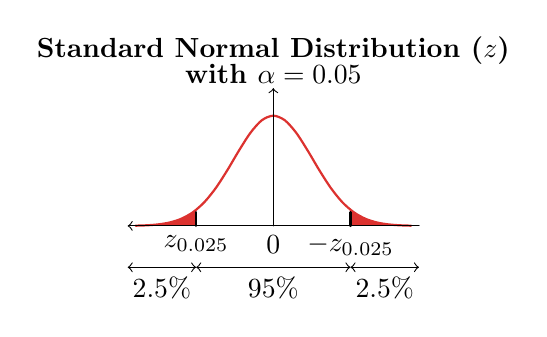
\begin{tikzpicture}[
                domain=-1:1,
                xscale=-0.5,
                yscale=3.5,
                smooth,
                line cap=round,
                line join=round,
            ]
            % Define critical z values
            \def\zcrit{1.96}

            % Fill left tail area (2.5%)
            \fill[custom_red] (-3.5,0) -- plot[domain=-3.5:-\zcrit] (\x, {0.4*exp(-(\x)^2/2)}) -- (-\zcrit,0) -- cycle;

            % Fill right tail area (2.5%)
            \fill[custom_red] (3.5,0) -- plot[domain=3.5:\zcrit] (\x, {0.4*exp(-(\x)^2/2)}) -- (\zcrit,0) -- cycle;

            % Draw the normal distribution curve
            \draw[thick, custom_red] plot[domain=-3.5:3.5] (\x, {0.4*exp(-(\x)^2/2)});

            % Mark the critical values
            \draw[thick] (-\zcrit,0) -- (-\zcrit,0.05);
            \node[below] at (-\zcrit,0) {$-z_{0.025}$};
            \draw[thick] (\zcrit,0) -- (\zcrit,0.05);
            \node[below] at (\zcrit,0) {$z_{0.025}$};

            \draw[<->] (-\zcrit, -0.15) -- (\zcrit, -0.15) node[midway, below] {$95\%$};
            \draw[<->] (-\zcrit, -0.15) -- (-3.7, -0.15) node[midway, below] {$2.5\%$};
            \draw[<->] (\zcrit, -0.15) -- (3.7, -0.15) node[midway, below] {$2.5\%$};


            % Draw horizontal axis
            \draw[->] (-3.7,0) -- (3.7,0) node[right] {};
            % Draw vertical axis
            \draw[->] (0,0) -- (0,0.5) node[above] {};
            % Mark the center
            \node[below] at (0,0) {$0$};
            % Title
            \node[above] at (0,0.55) {\textbf{Standard Normal Distribution ($z$)}};
            \node at (0,0.55) {\textbf{with $\alpha = 0.05$}};
        \end{tikzpicture}
    \end{center}
\end{definitionbox}

\begin{examplebox}{Find crtitical value for the 95\% CI}{}
    For a confidence interval of 95\%, we want to find the z-score that leaves 2.5\% in each tail of the normal distribution.\\
    We want to find the $z$-value where the cumulative area )from the left up to that $z-score$) is $1 - 0.025 = 0.975$.\\
    We look in the $z$-tables for the value closest to $0.975$ and read the row and column headers to find the $z$-value.\\
    The $z$-value is $1.96$.\\
\end{examplebox}

\begin{examplebox}{Find the 95\% confidence interval for the population mean $\mu$ given}{}
    A dataset of 103 students, of whom 71 pay rent, was used to estimate the average weekly rent $\mu$.
    \begin{itemize}
        \item \textbf{Point estimate}: the sample mean $\bar{X} \approx 546.239$.
        \item \textbf{Sample standard deviation}: $s \approx 187.862$.
        \item \textbf{Sample size}: $n = 71$.
    \end{itemize}
    Confidence Interval is given by:
    $$\bar{X} \pm z_{\alpha/2} \times \frac{s}{\sqrt{n}}\Rightarrow 546.239 \pm 1.96 \times \frac{187.862}{\sqrt{71}}$$
    where $z_{\alpha/2} = 1.96$ for a 95\% confidence level.The resulting confidence interval is:
    $$(502.541, 589.938)$$
    \textbf{Interpretation}: We are 95\% confident that the true mean weekly rent for all NUI Galway students (population) is roughly 503 to 590 euros.
\end{examplebox}
\subsubsection{Higher Confidence Levels means Wider Intervals}
\begin{itemize}
    \item To achieve a \textbf{higher confidence level}, we need to increase the critical value $z_{\alpha/2}$, which in turn increases the margin of error.
    \item This results in a wider confidence interval, which means we are more certain that the true population parameter lies within that interval.
    \item Conversely a \textbf{lower confidence level} results in a smaller critical value, leading to a narrower confidence interval.
\end{itemize}
\pagebreak
\subsubsection{CI with large $\boldsymbol{n}$, and $\boldsymbol{\sigma}$ unknown}
The $z$-based critical interval is given as:
$$\bar{X} \pm z_{\alpha/2} \times \frac{\sigma}{\sqrt{n}}$$
where $z_{\alpha/2}$ is the critical value from the standard normal distribution.
However, if the population standard deviation $\sigma$ is unknown, we can use the sample standard deviation $s$ as an estimate.\\
This gives us the following confidence interval:
$$\bar{X} \pm z_{\alpha/2} \times \frac{s}{\sqrt{n}}$$
\textbf{Interpretation}: around 95\% of all possible 95\% confidence intervals will contain the true population mean $\mu$. We can visualize that if we drew many repeated samples, sample means will form an overlapping $\mu$ and a small fraction will not.

\subsubsection{Confidence Intervals with small $n$ and $\sigma$ unknown}
\begin{conceptbox}{Why the $t-$distribution}{}
    When the sample size is small ($n < 30$) and the population standard deviation $\sigma$ is unknown, simply substituting the sample standard deviation $s$ no longer suffices because the standard error is itself estimated with more uncertainty.\\[2ex]
    The $\textbf{t-distributution has thicker}$ tails than the normal distributution. This extra "fatness" in the tails accounts for the additional uncertainty in using $s$ instead of $\sigma$.
    \begin{center}
        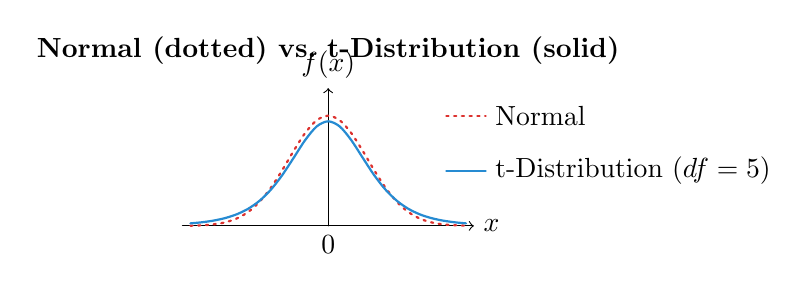
\begin{tikzpicture}[
            domain=-3.5:3.5,
            xscale=0.5,
            yscale=3.5,
            smooth,
            line cap=round,
            line join=round
        ]
            % Draw axes
            \draw[->] (-3.7,0) -- (3.7,0) node[right] {$x$};
            \draw[->] (0,0) -- (0,0.5) node[above] {$f(x)$};
            \node[below] at (0,0) {$0$};
        
            % Plot the Normal Distribution (dotted red)
            \draw[dotted, thick, custom_red] plot (\x, {0.4*exp(-(\x)^2/2)});
        
            % Plot the t-Distribution (solid blue) for df = 5.
            % The t-density: f(t) = (8/(3*pi*sqrt(5)))*(1+t^2/5)^(-3)
            \draw[thick, custom_blue] plot (\x, {(8/(3*3.14159*sqrt(5)))*((1+(\x)^2/5)^(-3))});
        
            % Title and legend
            \node[above] at (0,0.55) {\textbf{Normal (dotted) vs.\ t-Distribution (solid)}};
        
            % Legend (placed at the top-right)
            \begin{scope}[shift={(3,0.4)}]
                \draw[dotted, thick, custom_red] (0,0) -- (1,0);
                \node[right] at (1,0) {Normal};
                \draw[thick, custom_blue] (0,-0.2) -- (1,-0.2);
                \node[right] at (1,-0.2) {t-Distribution ($df=5$)};
            \end{scope}
        \end{tikzpicture}        
    \end{center}
\end{conceptbox}

\end{document}
